% Title: gl2ps_renderer figure
% Creator: GL2PS 1.4.2, (C) 1999-2020 C. Geuzaine
% For: Octave
% CreationDate: Sat Sep 11 15:20:41 2021
\setlength{\unitlength}{1pt}
\begin{picture}(0,0)
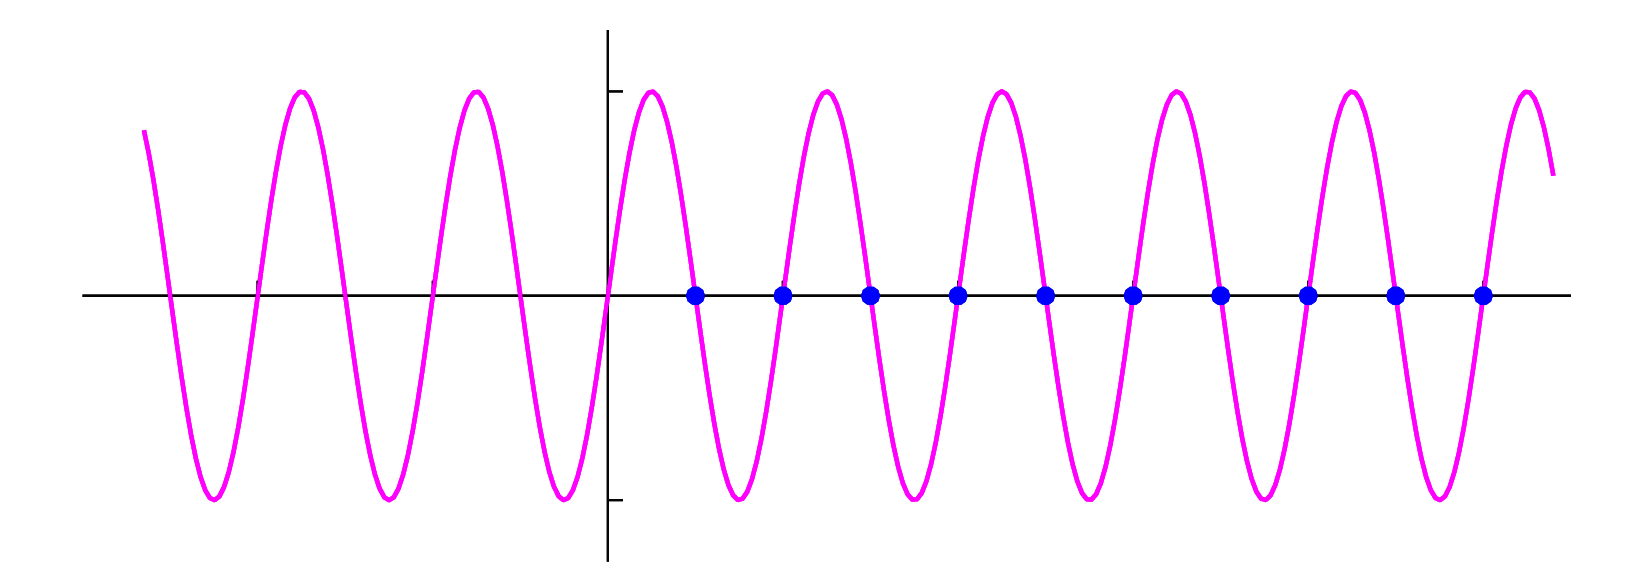
\includegraphics[width=14cm,height=5cm]{fig_exemplo_sequencia_por_funcao_sin}
\end{picture}%
\begin{picture}(396,141)(0,0)
\fontsize{10}{0}\selectfont\put(61.862,62.6597){\makebox(0,0)[t]{\textcolor[rgb]{0.15,0.15,0.15}{{-4}}}}
\fontsize{10}{0}\selectfont\put(103.881,62.6597){\makebox(0,0)[t]{\textcolor[rgb]{0.15,0.15,0.15}{{-2}}}}
\fontsize{10}{0}\selectfont\put(187.92,62.6597){\makebox(0,0)[t]{\textcolor[rgb]{0.15,0.15,0.15}{{2}}}}
\fontsize{10}{0}\selectfont\put(229.94,62.6597){\makebox(0,0)[t]{\textcolor[rgb]{0.15,0.15,0.15}{{4}}}}
\fontsize{10}{0}\selectfont\put(271.959,62.6597){\makebox(0,0)[t]{\textcolor[rgb]{0.15,0.15,0.15}{{6}}}}
\fontsize{10}{0}\selectfont\put(313.979,62.6597){\makebox(0,0)[t]{\textcolor[rgb]{0.15,0.15,0.15}{{8}}}}
\fontsize{10}{0}\selectfont\put(355.998,62.6597){\makebox(0,0)[t]{\textcolor[rgb]{0.15,0.15,0.15}{{10}}}}
\fontsize{10}{0}\selectfont\put(140.899,21.0727){\makebox(0,0)[r]{\textcolor[rgb]{0.15,0.15,0.15}{{-1}}}}
\fontsize{10}{0}\selectfont\put(140.899,119.195){\makebox(0,0)[r]{\textcolor[rgb]{0.15,0.15,0.15}{{1}}}}
\fontsize{10}{0}\selectfont\put(166.911,119.195){\makebox(0,0)[l]{\textcolor[rgb]{0,0,0}{{$f(x)$}}}}
\fontsize{10}{0}\selectfont\put(297.171,75.04){\makebox(0,0)[bl]{\textcolor[rgb]{0,0,0}{{$a_n$}}}}
\end{picture}
